\documentclass[11pt, letterpaper]{article}

\usepackage{multirow}
\usepackage{array}
\usepackage{booktabs}
\usepackage{graphicx}
\usepackage{floatrow}
\usepackage{longtable}
\usepackage{changepage}

\graphicspath{{/}}


\title{Sheet 2: HTML and CSS}
\date{2015-10-30}
\author{Creativity Through Code}

\addtolength{\oddsidemargin}{-.875in}
\addtolength{\evensidemargin}{-.875in}
\addtolength{\textwidth}{1.75in}

\addtolength{\topmargin}{-.875in}
\addtolength{\textheight}{1.75in}

\begin{document}
	\maketitle
	\newpage
	\begin{abstract}
		After the introducing the essentials of web development, we will be learning how we can create a beautiful static website using HTML and CSS.
	\end{abstract}
	\section{HTML}
		\textbf{HyperText Markup Language (HTML)} is the standard markup language used to created webpages. It is the building blocks of all websites and it provides the means to create structured documents by denoting structural semantics for text.
		\begin{longtable}{l l}
			\toprule
			Tag & Description \\\midrule
			\texttt{<!---...--->} & Defines a comment \\\midrule
			\texttt{<!DOCTYPE>} & Defines the document type \\\midrule
			\texttt{<a>} & Defines a hyperlink \\\midrule
			\texttt{<abbr>} & Defines an abbreviation or an acronym \\\midrule
			\texttt{<address>} & Defines contact information for the author/owner of a document \\\midrule
			\texttt{<area>} & Defines an area inside an image­map \\\midrule
			\texttt{<b>} & Defines bold text \\\midrule
			\texttt{<base>} & Specifies the base URL/target for all relative URLs in a document \\\midrule
			\texttt{<bdo>} & Overrides the current text direction \\\midrule
			\texttt{<blockquote>} & Defines a section that is quoted from another source \\\midrule
			\texttt{<body>} & Defines the document's body \\\midrule
			\texttt{<br>} & Defines a single link break \\\midrule
			\texttt{<button>} & Defines a clickable button \\\midrule
			\texttt{<caption>} & Defines a table caption \\\midrule
			\texttt{<cite>} & Defines the title of a work\\\midrule
			\texttt{<code>} & Defines a piece of computer code\\\midrule
			\texttt{<col>} & Specifies column properties for each column within a \texttt{<colgroup>} element\\\midrule
			\texttt{<colgroup>} & Specifies a group of one or more columns in a table for formatting\\\midrule
			\texttt{<dd>} & Defines a description/value of a term in a dsecription list\\\midrule
			\texttt{<del>} & Defines text that has been deleted from a document\\\midrule
			\texttt{<dfn>} & Represents the defining instance of a term \\\midrule
			\texttt{<div>} & Defines a section of a document\\\midrule
			\texttt{<dl>} & Defines a description list\\\midrule
			\texttt{<dt>} & Defines a term/name in a description list\\\midrule
			\texttt{<em>} & Defines emphasized text \\\midrule
			\texttt{<fieldset>} & Groups related elements in a form\\\midrule
			\texttt{<footer>} & Defines a footer for a document or section\\\midrule
			\texttt{<form>} & Defines a HTML form for user input\\\midrule
			\texttt{<h1> to <h6>} & Defines HTML headings\\\midrule
			\texttt{<head>} & Defines information about the document\\\midrule
			\texttt{<header>} & Defines a header for a document or section\\\midrule
			\texttt{<hr>} & Defines a thematic change in the content\\\midrule
			\texttt{<html>} & Defines the root of an HTML document\\\midrule
			\texttt{<i>} & Defines a part of text in italics\\\midrule
			\texttt{<iframe>} & Defines an inline frame\\\midrule
			\texttt{<img>} & Defines an image\\\midrule
			\texttt{<input>} & Defines an input control\\\midrule
			\texttt{<ins>} & Defines a text that has been inserted into a document\\\midrule
			\texttt{<kbd>} & Defines keyboard input\\\midrule
			\texttt{<labe>} & Defines a label for an \texttt{<input>} element\\\midrule
			\texttt{<legend>} & Defines a cptaion for a \texttt{<fieldset>} element\\\midrule
			\texttt{<li>} & Defines a list item\\\midrule
			\texttt{<link>} & Defines relationship between document and external resource\\\midrule
			\texttt{<map>} & Defines a client-side image-map\\\midrule
			\texttt{<menu>} & Defines a list/menu of commands\\\midrule
			\texttt{<menuitem>} & Defines a menu/command item\\\midrule
			\texttt{<meta>} & Defines metadata about an HTML document\\\midrule
			\texttt{<meter>} & Defines a scalar measurement within a known range\\\midrule
			\texttt{<nav>} & Defines navigation links\\\midrule
			\texttt{<noscript>} & Defines an alternate content for users\\\midrule
			\texttt{<object>} & Defines an embedded object\\\midrule
			\texttt{<ol>} & Defines an ordered list\\\midrule
			\texttt{<optgroup>} & Defines a group of related option in a drop-down list\\\midrule
			\texttt{<option>} & Defines an option in a drop-down list\\\midrule
			\texttt{<p>} & Defines a paragraph\\\midrule
			\texttt{<param>} & Defines a parameter for an object\\\midrule
			\texttt{<pre>} & Defines preformatted text\\\midrule
			\texttt{<q>} & Defines a short quotation\\\midrule
			\texttt{<s>} & Defines text that is no longer correct\\\midrule
			\texttt{<samp>} & Defines sample output from a computer program\\\midrule
			\texttt{<script>} & Defines a client-side script\\\midrule
			\texttt{<select>} & Defines a drop-down list\\\midrule
			\texttt{<small>} & Defines smaller text\\\midrule
			\texttt{<span>} & Defines a section in a document\\\midrule
			\texttt{<strong>} & Defines important text\\\midrule
			\texttt{<stlye>} & Defines style information for a document\\\midrule
			\texttt{<sub>} & Defines subscripted text\\\midrule
			\texttt{<sup>} & Defines superscripted text\\\midrule
			\texttt{<table>} & Defines a table\\\midrule
			\texttt{<tbody>} & Groups a body content in a table\\\midrule
			\texttt{<td>} & Defines a cell in a table\\\midrule
			\texttt{<textarea>} & Defines a multiline input control\\\midrule
			\texttt{<tfoot>} & Groups the footer content in table\\\midrule
			\texttt{<th>} & Defines a header cell in a table\\\midrule
			\texttt{<thead>} & Groups the header content in a table\\\midrule
			\texttt{<title>} & Defines a title for the document\\\midrule
			\texttt{<tr>} & Defines a row in a table\\\midrule
			\texttt{<u>} & Defines underlined text\\\midrule
			\texttt{<ul>} & Defines an unordered list\\\midrule
			\texttt{<var>} & Defines a variable\\
			\bottomrule
			\caption{Tag Descriptions}
		\end{longtable}
	\section{CSS}
		\subsection{Introduction}
		\textbf{Cascading Style Sheets (CSS)} is a style sheet language used for describing the presention of a document/webpage written in a markup language. It is designed primarily to enable the separation of document content from document presention, including aspects such as layout, colors, and fonts. In summary, the webpage content and structure is defined by \textbf{HTML} and the webpage presentation is defined by \textbf{CSS}.
		
		\subsection{Color Properties}
			\begin{longtable}{p{5cm} p{10cm}}
				\toprule
				Property & Description \\\midrule 
				\texttt{color} & Sets the color of text \\\midrule
				\texttt{opacity} & Sets the opacity level for an element \\\bottomrule
			\end{longtable}
		
		\subsection{Background and Border Properties}
			\begin{longtable}{p{5cm} p{10cm}}
				\toprule
				Property & Description \\\midrule 
				\texttt{background} & A shorthand property for setting all the background properties in one declaration \\\midrule
				\texttt{background-attachment} & Sets whether a background image is fixed or scrolls with the rest of the page \\\midrule
				\texttt{background-blend-mode} & Specifies the blending mode of each background layer (color/image) \\\midrule 
				\texttt{background-color} & Specifies the background color of an element \\\midrule
				\texttt{background-image} & Specifies one or more background images for an element \\\midrule
				\texttt{background-position} & Specifies the position of a background image \\\midrule
				\texttt{background-repeat} & Sets how a background image will be repeated \\\midrule
				\texttt{background-clip} & Specifies the painting area of the background \\\midrule
				\texttt{background-origin} & Specifies where the background image(s) is/are positioned \\\midrule
				\texttt{background-size} & Specifies the size of the background image(s) \\\midrule
				\texttt{border} & Sets all the border properties in one declaration \\\midrule
				\texttt{border-bottom} & Sets all the bottom border properties in one declaration \\\midrule
				\texttt{border-bottom-color} & Sets the color of the bottom border \\\midrule 
				\texttt{border-bottom-left-radius} & Defines the shape of the border of the bottom-left corner \\\midrule
				\texttt{border-bottom-right-radius} & Defines the shape of the border of the bottom-right corner \\\midrule
				\texttt{border-bottom-style} & Sets the style of the bottom border \\\midrule
				\texttt{border-bottom-width} & Sets the width of the bottom border \\\midrule
				\texttt{border-color} & Sets the color of the four borders \\\midrule
				\texttt{border-image} & A shorthand property for setting all the border-image-* properties \\\midrule
				\texttt{border-image-outset} & Specifies the amount by which the border image area extends beyond the border box \\\midrule
				\texttt{border-image-repeat} & Specifies whether the border image should be repeated, rounded or stretched \\\midrule
				\texttt{border-image-slice} & Specifies how to slice the border image \\\midrule
				\texttt{border-image-source} & Specifies the path to the image to be used as a border \\\midrule
				\texttt{border-image-width} & Specifies the widths of the image-border \\\midrule
				\texttt{border-left} & Sets all the left border properties in one declaration \\\midrule
				\texttt{border-left-color} & Sets the color of the left border \\\midrule
				\texttt{border-left-style} & Sets the style of the left border \\\midrule
				\texttt{border-left-width} & Sets the width of the left border \\\midrule
				\texttt{border-radius} & A shorthand property for setting all the four border-*-radius properties \\\midrule
				\texttt{border-right} & Sets all the right border properties in one declaration \\\midrule
				\texttt{border-right-color} & Sets the color of the right border \\\midrule
				\texttt{border-right-style} & Sets the style of the right border \\\midrule
				\texttt{border-right-width} & Sets the width of the right border \\\midrule
				\texttt{border-style} & Sets the style of the four borders \\\midrule
				\texttt{border-top} & Sets all the top border properties in one declaration \\\midrule
				\texttt{border-top-color} & Sets the color of the top border \\\midrule
				\texttt{border-top-left-radius} & Defines the shape of the border of the top-left corner \\\midrule
				\texttt{border-top-right-radius} & Defines the shape of the border of the top-right corner \\\midrule
				\texttt{border-top-style} & Sets the style of the top border \\\midrule
				\texttt{border-top-width} & Sets the width of the top border \\\midrule
				\texttt{border-width} & Sets the width of the four borders \\\midrule
				\texttt{box-decoration-break} & Sets the behaviour of the background and border of an element at page-break, or, for in-line elements, at line-break. \\\midrule
				\texttt{box-shadow} & Attaches one or more drop-shadows to the box \\\bottomrule
			\end{longtable}
		
		\subsection{Basic Box Properties}
			\begin{longtable}{p{5cm} p{10cm}}
				\toprule
				Property & Description \\\midrule 
				\texttt{bottom} & Specifies the bottom position of a positioned element \\\midrule
				\texttt{clear} & Specifies which sides of an element where other floating elements are not allowed \\\midrule
				\texttt{clip} & Clips an absolutely positioned element \\\midrule
				\texttt{display} & Specifies how a certain HTML element should be displayed \\\midrule
				\texttt{float} & Specifies whether or not a box should float \\\midrule
				\texttt{height} & Sets the height of an element \\\midrule
				\texttt{left} & Specifies the left position of a positioned element \\\midrule
				\texttt{margin} & Sets all the margin properties in one declaration \\\midrule
				\texttt{margin-bottom} & Sets the bottom margin of an element \\\midrule
				\texttt{margin-left} & Sets the left margin of an element \\\midrule
				\texttt{margin-right} & Sets the right margin of an element \\\midrule
				\texttt{margin-top} & Sets the top margin of an element \\\midrule
				\texttt{max-height} & Sets the maximum height of an element \\\midrule
				\texttt{max-width} & Sets the maximum width of an element \\\midrule
				\texttt{min-height} & Sets the minimum height of an element \\\midrule
				\texttt{min-width} & Sets the minimum width of an element \\\midrule
				\texttt{overflow} & Specifies what happens if content overflows an element's box \\\midrule
				\texttt{overflow-x} & Specifies whether or not to clip the left/right edges of the content, if it overflows the element's content area \\\midrule
				\texttt{overflow-y} & Specifies whether or not to clip the top/bottom edges of the content, if it overflows the element's content area \\\midrule
				\texttt{padding} & Sets all the padding properties in one declaration \\\midrule
				\texttt{padding-bottom} & Sets the bottom padding of an element \\\midrule
				\texttt{padding-left} & Sets the left padding of an element \\\midrule
				\texttt{padding-right} & Sets the right padding of an element \\\midrule
				\texttt{padding-top} & Sets the top padding of an element \\\midrule
				\texttt{position} & Specifies the type of positioning method used for an element (static, relative, absolute or fixed) \\\midrule
				\texttt{right} & Specifies the right position of a positioned element \\\midrule
				\texttt{top} & Specifies the top position of a positioned element \\\midrule
				\texttt{visibility} & Specifies whether or not an element is visible \\\midrule
				\texttt{width} & Sets the width of an element \\\midrule
				\texttt{vertical-align} & Sets the vertical alignment of an element \\\midrule
				\texttt{z-index} & Sets the stack order of a positioned element \\\midrule
			\end{longtable}
		
		\subsection{Flexible Box Layout}
			\begin{longtable}{p{5cm} p{10cm}}
				\toprule
				Property & Description \\\midrule 
				\texttt{align-content} & Specifies the alignment between the lines inside a flexible container when the items do not use all available space \\\midrule
				\texttt{align-items} & Specifies the alignment for items inside a flexible container \\\midrule
				\texttt{align-self} & Specifies the alignment for selected items inside a flexible container \\\midrule
				\texttt{flex} & Specifies the length of the item, relative to the rest \\\midrule
				\texttt{flex-basis} & Specifies the initial length of a flexible item \\\midrule
				\texttt{flex-direction} & Specifies the direction of the flexible items \\\midrule
				\texttt{flex-flow} & A shorthand property for the flex-direction and the flex-wrap properties \\\midrule
				\texttt{flex-grow} & Specifies how much the item will grow relative to the rest \\\midrule
				\texttt{flex-shrink} & Specifies how the item will shrink relative to the rest \\\midrule
				\texttt{flex-wrap} & Specifies whether the flexible items should wrap or not \\\midrule
				\texttt{justify-content} & Specifies the alignment between the items inside a flexible container when the items do not use all available space \\\midrule
				\texttt{order} & Sets the order of the flexible item, relative to the rest \\\midrule
			\end{longtable}

		\subsection{Text Properties}
			\begin{longtable}{p{5cm} p{10cm}}
				\toprule
				Property & Description \\\midrule
				\texttt{hanging-punctuation} & Specifies whether a punctuation character may be placed outside the line box \\\midrule
				\texttt{hyphens} & Sets how to split words to improve the layout of paragraphs \\\midrule
				\texttt{letter-spacing} & Increases or decreases the space between characters in a text \\\midrule
				\texttt{line-break} & Specifies how/if to break lines \\\midrule
				\texttt{line-height} & Sets the line height \\\midrule
				\texttt{overflow-wrap} & Specifies whether or not the browser may break lines within words in order to prevent overflow (when a string is too long to fit its containing box)\\\midrule
				\texttt{tab-size} & Specifies the length of the tab-character \\\midrule
				\texttt{text-align} & Specifies the horizontal alignment of text \\\midrule
				\texttt{text-align-last} & Describes how the last line of a block or a line right before a forced line break is aligned when text-align is ``justify'' \\\midrule
				\texttt{text-combine-upright} & Specifies the combination of multiple characters into the space of a single character \\\midrule
				\texttt{text-indent} & Specifies the indentation of the first line in a text-block \\\midrule
				\texttt{text-justify} & Specifies the justification method used when text-align is ``justify'' \\\midrule
				\texttt{text-transform} & Controls the capitalization of text \\\midrule
				\texttt{white-space} & Specifies how white-space inside an element is handled \\\midrule
				\texttt{word-break} & Specifies line breaking rules for non-CJK scripts \\\midrule
				\texttt{word-spacing} & Increases or decreases the space between words in a text \\\midrule
				\texttt{word-wrap} & Allows long, unbreakable words to be broken and wrap to the next line \\\midrule
			\end{longtable}

		\subsection{Text Decoration Properties}
			\begin{longtable}{p{5cm} p{10cm}}
				\toprule
				Property & Description \\\midrule 
				\texttt{text-decoration} & Specifies the decoration added to text \\\midrule
				\texttt{text-decoration-color} & Specifies the color of the text-decoration \\\midrule
				\texttt{text-decoration-line} & Specifies the type of line in a text-decoration \\\midrule
				\texttt{text-decoration-style} & Specifies the style of the line in a text decoration \\\midrule
				\texttt{text-shadow} & Adds shadow to text \\\midrule
				\texttt{text-underline-position} & Specifies the position of the underline which is set using the text-decoration property \\\midrule
			\end{longtable}

		\subsection{Font Properties}
			\begin{longtable}{p{5cm} p{10cm}}
				\toprule
				Property & Description \\\midrule 
				\texttt{@font-face} & A rule that allows websites to download and use fonts other than the ``web-safe'' fonts \\\midrule
				\texttt{@font-feature-values} & Allows authors to use a common name in font-variant-alternate for feature activated differently in OpenType \\\midrule
				\texttt{font} & Sets all the font properties in one declaration \\\midrule
				\texttt{font-family} & Specifies the font family for text \\\midrule
				\texttt{font-feature-settings} & Allows control over advanced typographic features in OpenType fonts \\\midrule
				\texttt{font-kerning} & Controls the usage of the kerning information (how letters are spaced) \\\midrule
				\texttt{font-language-override} & Controls the usage of language-specific glyphs in a typeface \\\midrule
				\texttt{font-size} & Specifies the font size of text \\\midrule
				\texttt{font-size-adjust} & Preserves the readability of text when font fallback occurs \\\midrule
				\texttt{font-stretch} & Selects a normal, condensed, or expanded face from a font family \\\midrule
				\texttt{font-style} & Specifies the font style for text \\\midrule
				\texttt{font-synthesis} & Controls which missing typefaces (bold or italic) may be synthesized by the browser \\\midrule
				\texttt{font-variant} & Specifies whether or not a text should be displayed in a small-caps font \\\midrule
				\texttt{font-variant-alternates} & Controls the usage of alternate glyphs associated to alternative names defined in @font-feature-values \\\midrule
				\texttt{font-variant-caps} & Controls the usage of alternate glyphs for capital letters \\\midrule
				\texttt{font-variant-east-asian} & Controls the usage of alternate glyphs for East Asian scripts (e.g Japanese and Chinese) \\\midrule
				\texttt{font-variant-ligatures} & Controls which ligatures and contextual forms are used in textual content of the elements it applies to \\\midrule
				\texttt{font-variant-numeric} & Controls the usage of alternate glyphs for numbers, fractions, and ordinal markers \\\midrule
				\texttt{font-variant-position} & Controls the usage of alternate glyphs of smaller size positioned as superscript or subscript regarding the baseline of the font \\\midrule
				\texttt{font-weight} & Specifies the weight of a font \\\midrule
			\end{longtable}

		\subsection{Writing Modes Properties}
			\begin{longtable}{p{5cm} p{10cm}}
				\toprule
				Property & Description \\\midrule 
				\texttt{direction} & Specifies the text direction/writing direction \\\midrule
				\texttt{text-orientation} & Defines the orientation of the text in a line \\\midrule
				\texttt{text-combine-upright} & Specifies the combination of multiple characters into the space of a single character \\\midrule
				\texttt{unicode-bidi} & Used together with the direction property to set or return whether the text should be overridden to support multiple languages in the same document \\\midrule
				\texttt{writing-mode} & \\\midrule
			\end{longtable}

		\subsection{Table Properties}
			\begin{longtable}{p{5cm} p{10cm}}
				\toprule
				Property & Description \\\midrule 
				\texttt{border-collapse} & Specifies whether or not table borders should be collapsed \\\midrule
				\texttt{border-spacing} & Specifies the distance between the borders of adjacent cells \\\midrule
				\texttt{caption-side} & Specifies the placement of a table caption \\\midrule
				\texttt{empty-cells} & Specifies whether or not to display borders and background on empty cells in a table \\\midrule
				\texttt{table-layout} & Sets the layout algorithm to be used for a table \\\midrule
			\end{longtable}

		\subsection{Lists and Counters Properties}
			\begin{longtable}{p{5cm} p{10cm}}
				\toprule
				Property & Description \\\midrule 
				\texttt{counter-increment} & Increments one or more counters \\\midrule
				\texttt{counter-reset} & Creates or resets one or more counters \\\midrule
				\texttt{list-style} & Sets all the properties for a list in one declaration \\\midrule
				\texttt{list-style-image} & Specifies an image as the list-item marker \\\midrule
				\texttt{list-style-position} & Specifies if the list-item markers should appear inside or outside the content flow \\\midrule
				\texttt{list-style-type} & Specifies the type of list-item marker \\\midrule
			\end{longtable}

		\subsection{Animation Properties}
			\begin{longtable}{p{5cm} p{10cm}}
				\toprule
				Property & Description \\\midrule 
				\texttt{@keyframes} & Specifies the animation code \\\midrule
				\texttt{animation} & A shorthand property for all the animation properties (except animation-play-state and animation-fill-mode) \\\midrule
				\texttt{animation-delay} & Specifies a delay for the start of an animation \\\midrule
				\texttt{animation-direction} & Specifies whether or not the animation should play in reverse on alternate cycles \\\midrule
				\texttt{animation-duration} & Specifies how many seconds or milliseconds an animation takes to complete one cycle \\\midrule
				\texttt{animation-fill-mode} & Specifies a style for the element when the animation is not playing (when it is finished, or when it has a delay) \\\midrule
				\texttt{animation-iteration-count} & Specifies the number of times an animation should be played \\\midrule
				\texttt{animation-name} & Specifies the name of the @keyframes animation \\\midrule
				\texttt{animation-play-state} & Specifies whether the animation is running or paused \\\midrule
				\texttt{animation-timing-function} & Specifies the speed curve of an animation \\\midrule
			\end{longtable}

		\subsection{Transform Properties}
			\begin{longtable}{p{5cm} p{10cm}}
				\toprule
				Property & Description \\\midrule 
				\texttt{backface-visibility} & Defines whether or not an element should be visible when not facing the screen \\\midrule
				\texttt{perspective} & Specifies the perspective on how 3D elements are viewed \\\midrule
				\texttt{perspective-origin} & Specifies the bottom position on 3D elements \\\midrule
				\texttt{transform} & Applies a 2D or 3D transformation to an element \\\midrule
				\texttt{transform-origin} & Allows you to change the position on transformed elements \\\midrule
				\texttt{transform-style} & Specifies how nested elements are rendered in 3D space \\\midrule
			\end{longtable}

		\subsection{Transitions Properties}
			\begin{longtable}{p{5cm} p{10cm}}
				\toprule
				Property & Description \\\midrule 
				\texttt{transition} & A shorthand property for setting the four transition properties \\\midrule
				\texttt{transition-property} & Specifies the name of the CSS property the transition effect is for \\\midrule
				\texttt{transition-duration} & Specifies how many seconds or milliseconds a transition effect takes to complete \\\midrule
				\texttt{transition-timing-function} & Specifies the speed curve of the transition effect \\\midrule
				\texttt{transition-delay} & Specifies when the transition effect will start \\\midrule
			\end{longtable}

		\subsection{Basic User Interface Properties}
			\begin{longtable}{p{5cm} p{10cm}}
				\toprule
				Property & Description \\\midrule 
				\texttt{box-sizing} & Tells the browser what the sizing properties (width and height) should include \\\midrule
				\texttt{content} & Used with the :before and :after pseudo-elements, to insert generated content \\\midrule
				\texttt{cursor} & Specifies the type of cursor to be displayed \\\midrule
				\texttt{ime-mode} & Controls the state of the input method editor for text fields \\\midrule
				\texttt{nav-down} & Specifies where to navigate when using the arrow-down navigation key \\\midrule
				\texttt{nav-index} & Specifies the tabbing order for an element \\\midrule
				\texttt{nav-left} & Specifies where to navigate when using the arrow-left navigation key \\\midrule
				\texttt{nav-right} & Specifies where to navigate when using the arrow-right navigation key \\\midrule
				\texttt{nav-up} & Specifies where to navigate when using the arrow-up navigation key \\\midrule
				\texttt{outline} & Sets all the outline properties in one declaration \\\midrule
				\texttt{outline-color} & Sets the color of an outline \\\midrule
				\texttt{outline-offset} & Offsets an outline, and draws it beyond the border edge \\\midrule
				\texttt{outline-style} & Sets the style of an outline \\\midrule
				\texttt{outline-width} & Sets the width of an outline \\\midrule
				\texttt{resize} & Specifies whether or not an element is resizable by the user \\\midrule
				\texttt{text-overflow} & Specifies what should happen when text overflows the containing element \\\midrule
			\end{longtable}

		\subsection{Multi-column Layout Properties}
			\begin{longtable}{p{5cm} p{10cm}}
				\toprule
				Property & Description \\\midrule 
				\texttt{break-after} & Specifies the page-, column-, or region-break behavior after the generated box \\\midrule
				\texttt{break-before} & Specifies the page-, column-, or region-break behavior before the generated box \\\midrule
				\texttt{break-inside} & Specifies the page-, column-, or region-break behavior inside the generated box \\\midrule
				\texttt{column-count} & Specifies the number of columns an element should be divided into \\\midrule
				\texttt{column-fill} & Specifies how to fill columns \\\midrule
				\texttt{column-gap} & Specifies the gap between the columns \\\midrule
				\texttt{column-rule} & A shorthand property for setting all the column-rule-* properties \\\midrule
				\texttt{column-rule-color} & Specifies the color of the rule between columns \\\midrule
				\texttt{column-rule-style} & Specifies the style of the rule between columns \\\midrule
				\texttt{column-rule-width} & Specifies the width of the rule between columns \\\midrule
				\texttt{column-span} & Specifies how many columns an element should span across \\\midrule
				\texttt{column-width} & Specifies the width of the columns \\\midrule
				\texttt{columns} & A shorthand property for setting column-width and column-count \\\midrule
				\texttt{widows} & Sets the minimum number of lines that must be left at the top of a page when a page break occurs inside an element \\\midrule
			\end{longtable}

		\subsection{Paged Media}
			\begin{longtable}{p{5cm} p{10cm}}
				\toprule
				Property & Description \\\midrule 
				\texttt{orphans} & Sets the minimum number of lines that must be left at the bottom of a page when a page break occurs inside an element \\\midrule
				\texttt{page-break-after} & Sets the page-breaking behavior after an element \\\midrule
				\texttt{page-break-before} & Sets the page-breaking behavior before an element \\\midrule
				\texttt{page-break-inside} & Sets the page-breaking behavior inside an element \\\midrule
			\end{longtable}

		\subsection{Generated Content for Paged Media}
			\begin{longtable}{p{5cm} p{10cm}}
				\toprule
				Property & Description \\\midrule 
				\texttt{marks} & Adds crop and/or cross marks to the document \\\midrule
				\texttt{quotes} & Sets the type of quotation marks for embedded quotations \\\midrule
			\end{longtable}

		\subsection{Filter Effects Properties}
			\begin{longtable}{p{5cm} p{10cm}}
				\toprule
				Property & Description \\\midrule 
				\texttt{filter} & Defines effects (e.g. blurring or color shifting) on an element before the element is displayed \\\midrule
			\end{longtable}

		\subsection{Image Values and Replaced Content}
			\begin{longtable}{p{5cm} p{10cm}}
				\toprule
				Property & Description \\\midrule 
				\texttt{image-orientation} & Specifies a rotation in the right or clockwise direction that a user agent applies to an image (This property is likely going to be deprecated and its functionality moved to HTML) \\\midrule
				\texttt{image-rendering} & Gives a hint to the browser about what aspects of an image are most important to preserve when the image is scaled \\\midrule
				\texttt{image-resolution} & Specifies the intrinsic resolution of all raster images used in/on the element \\\midrule
				\texttt{object-fit} & Specifies how the contents of a replaced element should be fitted to the box established by its used height and width \\\midrule
				\texttt{object-position} & Specifies the alignment of the replaced element inside its box \\\midrule
			\end{longtable}

		\subsection{Masking Properties}
			\begin{longtable}{p{5cm} p{10cm}}
				\toprule
				Property & Description \\\midrule 
				\texttt{mask} &  \\\midrule
				\texttt{mask-type} &  \\\midrule
			\end{longtable}

		\subsection{Speech Properties}
			\begin{longtable}{p{5cm} p{10cm}}
				\toprule
				Property & Description \\\midrule 
				\texttt{mark} & A shorthand property for setting the mark-before and mark-after properties \\\midrule
				\texttt{mark-after} & Allows named markers to be attached to the audio stream \\\midrule
				\texttt{mark-before} & Allows named markers to be attached to the audio stream \\\midrule
				\texttt{phonemes} & Specifies a phonetic pronunciation for the text contained by the corresponding element \\\midrule
				\texttt{rest} & A shorthand property for setting the rest-before and rest-after properties \\\midrule
				\texttt{rest-after} & Specifies a rest or prosodic boundary to be observed after speaking an element's content \\\midrule
				\texttt{rest-before} & Specifies a rest or prosodic boundary to be observed before speaking an element's content \\\midrule
				\texttt{voice-balance} & Specifies the balance between left and right channels \\\midrule
				\texttt{voice-duration} & Specifies how long it should take to render the selected element's content \\\midrule
				\texttt{voice-pitch} & Specifies the average pitch (a frequency) of the speaking voice \\\midrule
				\texttt{voice-pitch-range} & Specifies variation in average pitch \\\midrule
				\texttt{voice-rate} & Controls the speaking rate \\\midrule
				\texttt{voice-stress} & Indicates the strength of emphasis to be applied \\\midrule
				\texttt{voice-volume} & Refers to the amplitude of the waveform output by the speech synthesises \\\midrule
			\end{longtable}

		\subsection{Marquee Properties}
			\begin{longtable}{p{5cm} p{10cm}}
				\toprule
				Property & Description \\\midrule 
				\texttt{marquee-direction} & Sets the direction of the moving content \\\midrule
				\texttt{marquee-play-count} & Sets how many times the content move \\\midrule
				\texttt{marquee-speed} & Sets how fast the content scrolls \\\midrule
				\texttt{marquee-style} & Sets the style of the moving content \\\midrule
			\end{longtable}

	\section{Layout}
		With the release of \textbf{HTML 5}, specific layout components were introduced to structurally define a webpage better.\\\\

		\centering
		\begin{tabular}{m{7cm} m{8cm}}
			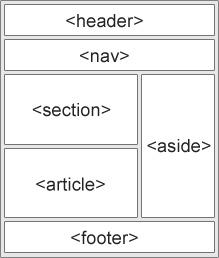
\includegraphics[scale = 1.3]{layout} & 
			\begin{tabular}{l p{5cm} l}
				\toprule
				Tag & Definition \\\midrule
				\texttt{<header>} & Defines a header for a document or a section \\\midrule
				\texttt{<nav>} & Defines a container for navigation links \\\midrule
				\texttt{<section>} & Defines a section in a document \\\midrule
				\texttt{<aside>} & Defines a sidebar (content aside from the container) \\\midrule
				\texttt{<details>} & Defines additional details \\\midrule
				\texttt{<summary>} & Defines a heading for the details element \\
				\bottomrule
			\end{tabular}
		\end{tabular}
\end{document}